%%%%%%%%%%%%%%%%%%%%%%%%%%%%%%%%%%%%%%%%%%%%%%%%%%%%%%%%%%%%%%%%%%%%%%%
%%%
%%%    【非公式】東京理科大学大学院 創域理工学研究科 機械航空宇宙工学専攻
%%%                         修士論文要旨 テンプレート
%%%
%%%                                  v1.2.0 Yuki MATSUKAWA 21 Dec. 2022
%%%                                  v2.0.0 Yuki MATSUKAWA 25 Dec. 2023
%%%
%%%%%%%%%%%%%%%%%%%%%%%%%%%%%%%%%%%%%%%%%%%%%%%%%%%%%%%%%%%%%%%%%%%%%%%
\documentclass[a4paper,fleqn,11pt]{jreport}

\usepackage{abst}			%abstract style
\usepackage{epsf,color}
\usepackage{float}
\usepackage{subfigure}	
\usepackage{rotating}
\usepackage{lscape}	
\usepackage{bm}
\usepackage{multirow}		
\usepackage{multicol}
\pagestyle{empty}

\begin{document}

% 一行あたり文字数の指定
\mojiparline{35}
% 1ページあたり行数の指定
\linesparpage{30}

\begin{center}
\fontsize{12pt}{20pt}\selectfont
ここには修士論文のタイトルを入れます.\\ 一文字でも間違えたら受理されません.
\end{center}

\ 

\noindent
% 姓と名の間に全角スペース忘れずに %
\begin{flushright}
機械工学専攻 \qquad 姓姓 名名 \\
指導教員 \qquad 塚原 隆裕
\end{flushright}

\ 

% ここから書き始める %
アブストラクトアブストラクトアブストラクトアブストラクトアブストラクトアブストラクトアブストラクトアブストラクトアブストラクト
アブストラクトアブストラクトアブストラクトアブストラクトアブストラクトアブストラクトアブストラクトアブストラクトアブストラクト
アブストラクトアブストラクトアブストラクトアブストラクトアブストラクトアブストラクトアブストラクトアブストラクトアブストラクト
アブストラクトアブストラクトアブストラクトアブストラクトアブストラクトアブストラクトアブストラクトアブストラクトアブストラクト
アブストラクトアブストラクトアブストラクトアブストラクトアブストラクトアブストラクトアブストラクトアブストラクトアブストラクト
アブストラクトアブストラクトアブストラクトアブストラクトアブストラクトアブストラクトアブストラクトアブストラクトアブストラクト
アブストラクトアブストラクトアブストラクトアブストラクトアブストラクトアブストラクトアブストラクトアブストラクトアブストラクト.

アブストラクトアブストラクトアブストラクトアブストラクトアブストラクトアブストラクトアブストラクトアブストラクトアブストラクト
アブストラクトアブストラクトアブストラクトアブストラクトアブストラクトアブストラクトアブストラクトアブストラクトアブストラクト
アブストラクトアブストラクトアブストラクトアブストラクトアブストラクトアブストラクトアブストラクトアブストラクトアブストラクト
アブストラクトアブストラクトアブストラクトアブストラクトアブストラクトアブストラクトアブストラクトアブストラクトアブストラクト
アブストラクトアブストラクトアブストラクトアブストラクトアブストラクトアブストラクトアブストラクトアブストラクトアブストラクト
アブストラクトアブストラクトアブストラクトアブストラクトアブストラクトアブストラクトアブストラクトアブストラクトアブストラクト
アブストラクトアブストラクトアブストラクトアブストラクトアブストラクトアブストラクトアブストラクトアブストラクトアブストラクト.

\fref{fig:abst1}は虎,\fref{fig:abst2}も虎.
アブストラクトアブストラクトアブストラクトアブストラクトアブストラクトアブストラクトアブストラクトアブストラクトアブストラクト
アブストラクトアブストラクトアブストラクトアブストラクトアブストラクトアブストラクトアブストラクトアブストラクトアブストラクト
アブストラクトアブストラクトアブストラクトアブストラクトアブストラクトアブストラクトアブストラクトアブストラクトアブストラクト
アブストラクトアブストラクトアブストラクトアブストラクトアブストラクトアブストラクトアブストラクトアブストラクトアブストラクト
アブストラクトアブストラクトアブストラクトアブストラクトアブストラクトアブストラクトアブストラクトアブストラクトアブストラクト
アブストラクトアブストラクトアブストラクトアブストラクトアブストラクトアブストラクトアブストラクトアブストラクトアブストラクト
アブストラクトアブストラクトアブストラクトアブストラクトアブストラクトアブストラクトアブストラクトアブストラクトアブストラクト
アブストラクトアブストラクトアブストラクトアブストラクトアブストラクトアブストラクトアブストラクトアブストラクトアブストラクト
アブストラクトアブストラクトアブストラクトアブストラクトアブストラクトアブストラクトアブストラクトアブストラクトアブストラクト.

\begin{multicols}{2}
   	\begin{figure}[H]
   		\begin{center}
   		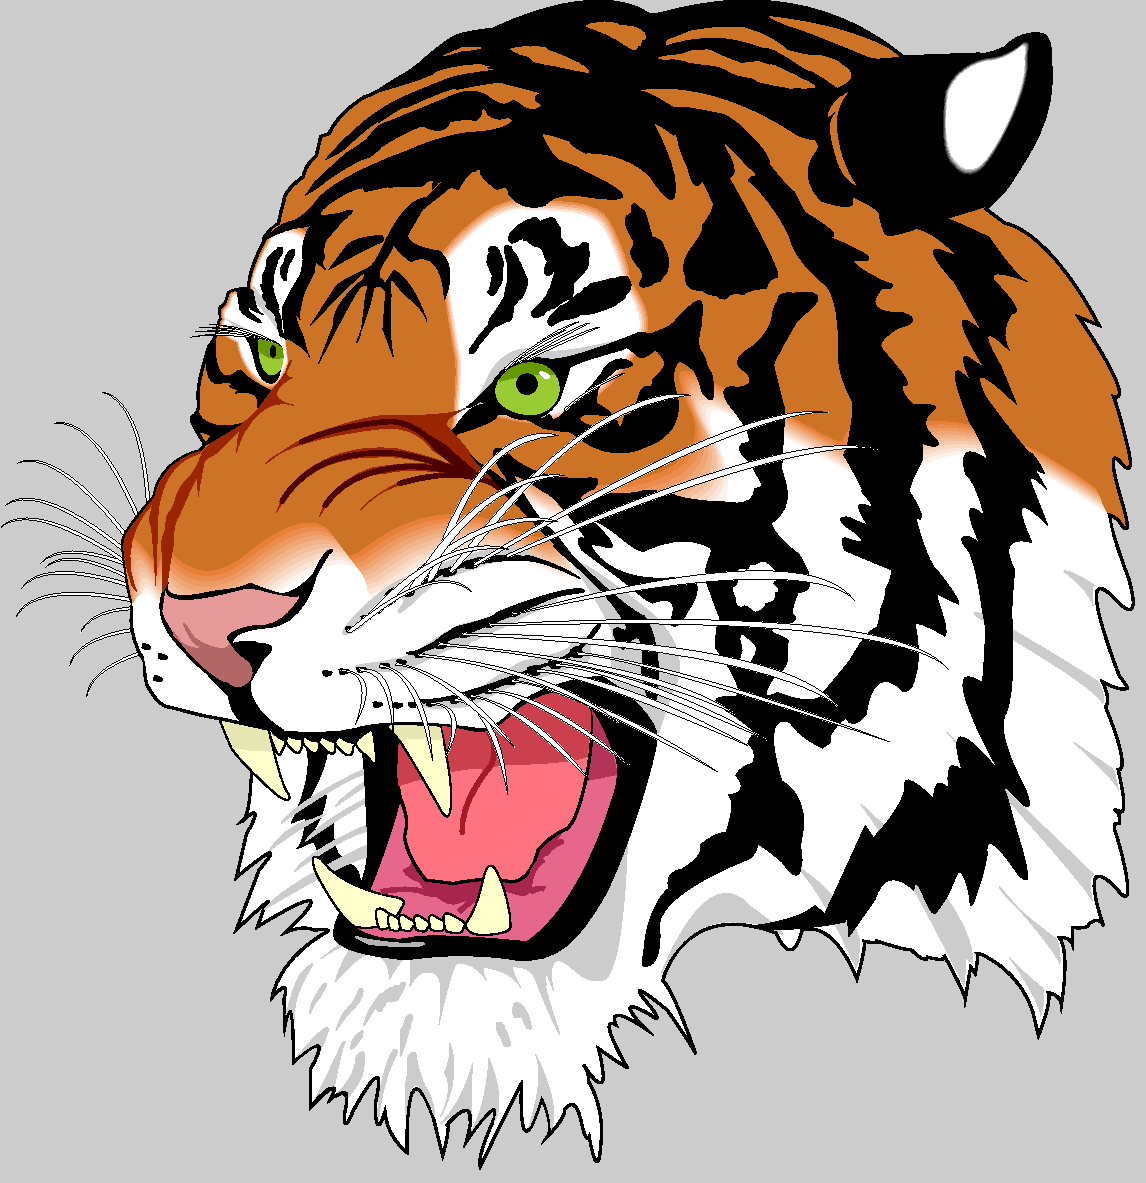
\includegraphics[width=0.6\columnwidth]{tiger.eps}
		\vspace{1.2cm}
   		\caption{Tiger 1.}
   		\label{fig:abst1}
   		\end{center}
   	\end{figure}

   	\begin{figure}[H]
   		\begin{center}
   		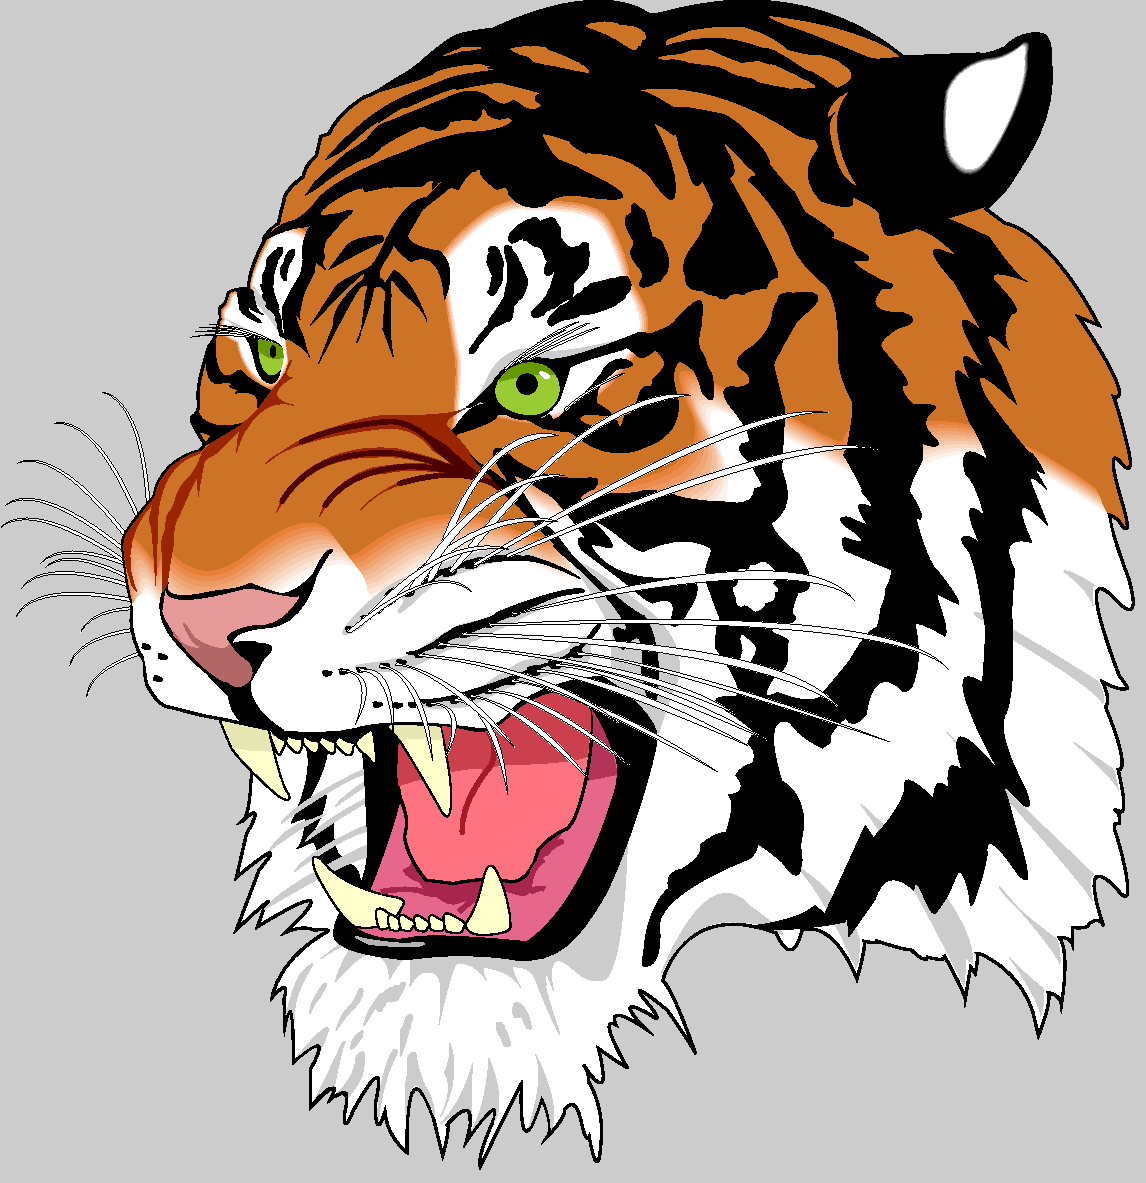
\includegraphics[width=0.6\columnwidth]{tiger.eps}
		\vspace{1.2cm}
   		\caption{Tiger 2.}
   		\label{fig:abst2}
   		\end{center}
   	\end{figure}
\end{multicols}


\end{document}
